%\documentclass[11pt,oneside]{uhthesis}
\documentclass[11pt,oneside]{report}
\usepackage{subfigure}
\usepackage[linesnumbered,lined,titlenumbered,ruled]{algorithm2e}
\usepackage{amsmath}
\usepackage{amssymb}
\usepackage{amsbsy}
\usepackage{mathpazo}
\usepackage{float}
\usepackage{braket}
\setlength {\marginparwidth }{3cm}
% \usepackage{todonotes}

\usepackage[spanish]{babel}
\usepackage{graphicx}

\usepackage{listings}
\usepackage{color}
\usepackage{booktabs}
\usepackage{multirow}
\usepackage{ragged2e}

%\floatstyle{ruled}
%\restylefloat{table}
\usepackage{listings}
\usepackage{color}

\definecolor{dkgreen}{rgb}{0,0.6,0}
\definecolor{gray}{rgb}{0.2,0,0}
\definecolor{mauve}{rgb}{0.58,0,0.82}

\lstset{language=Lisp,
	aboveskip=10mm,
	belowskip=10mm,
	showstringspaces=false,
	columns=flexible,
	basicstyle={\small\ttfamily},
	keywordstyle=\color{blue},
	commentstyle=\color{dkgreen},
	stringstyle=\color{mauve},
	breaklines=true,
	breakatwhitespace=true,
	tabsize=3,
	numbers=left, numberstyle=\tiny, stepnumber=1,firstnumber=1,
	numbersep=5pt
}

\renewcommand{\tablename}{Tabla}
\title{Un sistema para resolver variantes del Problema de Enrutamiento de Vehículos}
\author{Rodrigo García Gómez}
% \advisor{MSc. Fernando Rodríguez Flores}
% \coadvisor{}
%\degree{Licenciado en Ciencias de la Computación}
%\faculty{Facultad de Matemática y Computación}
\date{Noviembre de 2022}
%\logo{Graphics/uhlogo}

\renewcommand{\vec}[1]{\boldsymbol{#1}}
\newcommand{\diff}[1]{\ensuremath{\mathrm{d}#1}}

\begin{document}
\selectlanguage{spanish}

% \frontmatter
%\maketitle

%\begin{dedication}
	\textit{
		A mis padres,\\ 
		a mi hermano,\\
		a Alain, \\
		a Sinaile,\\
		a mi familia,\\
		a todos los que confiaron en mí cuando yo no creía.}
\end{dedication}
%\chapter*{Agradecimientos}\label{chapter:agradecimientos}

Un agradecimiento especial a mis padres, por estar siempre presentes en mi vida, por apoyarme y consentirme en todo momento.\\

A mi tía Marilín por acogerme como otra hija más durante esta etapa. \\

A Alain por ser el mejor maestro, ejemplo y compañero de viaje.\\

A Dayany Alfaro González por brindarme su amistad y las largas horas de estudio. \\

A Ashley Tejeda Meneses por siempre estar en los buenos y malos momentos. \\

A la familia cojimera, muchas gracias por abrirme sus puertas y ayudarme siempre.\\

A la profesora Celia Tamara González González por apostar por mí desde primer año, permitirme trabajar con ella y por apoyarme en todo momento, sobretodo en esta última etapa. \\ 

A José Jorge Rodríguez Salgado por la brillante idea que significó el punto de partida de esta tesis.\\

A mi tutor Fernando Rodríguez Flores por depositar su confianza en mí desde un inicio, por guiarme durante todo este proceso y regalarme sus conocimientos y consejos.\\




% Fernado




%\begin{opinion}	
	%El Problema de Enrutamiento de Vehículos (VRP) es uno de los problemas más estudiado dentro de la logística, por su importancia práctica y académica.  En nuestra facultad se han propuesto varias vías de solución para este tipo de problema, pero siempre usando algoritmos de optimización discreta.  Por otro lado, los algoritmos de optimización continua suelen tener mejores resultados y ser más rápidos que los discretos, ventajas estas que estaban vedadas al VRP...  hasta ahora.
	
	Con este trabajo se explora la posibilidad de convertir el espacio de soluciones discreto de un VRP a un espacio continuo sobre el que se puede aplicar cualquiera de los algoritmos de optimización continua existentes.  Para realizar esta transformación se usan técnicas de aprendizaje de máquinas.
	
	Creo que la palabra clave en este trabajo es aprendizaje, y no solo el que realizan los \textit{autoencoders} para convertir elementos de un espacio en elementos de otro, sino el que hemos realizado todos los involucrados en este proyecto.
	
	Para realizar esta tesis Dalianys tuvo que incursionar en (aprender) temas que no están incluidos en su plan de estudios, (aprender a) resolver creativamente problemas que aparecieron como parte del proceso de desarrollo y adquirir habilidades (aprender) relacionadas con la escritura de documentos científicos.
	
	Por otra parte, los demás involucrados también hemos aprendido: de la constancia y dedicación de Dalianys, de su independencia, y de su capacidad de búsqueda, organización, procesamiento y análisis de información científica.  Por todo eso, y por la trayectoria que ha tenido como estudiante y como alumna ayudante, considero que estamos en presencia de un excelente trabajo, que resume una excelente trayectoria, de una excelente profesional de la Ciencia de la Computación.
	
	\vspace{1cm}
	
	
	\begin{flushright}
		\underline{\hspace{6.5cm}}\\
		MSc. Fernando Raul Rodriguez Flores
		
		Facultad de Matemática y Computación
		
		Universidad de la Habana
		
		Noviembre, 2021
	\end{flushright}

\end{opinion}
\begin{abstract}
El problema de enrutamiento de vehículos (VRP) posee gran importancia académica e industrial. La cantidad de variantes que pueden existir es virtualmente infinita, limitada sólo por la imaginación humana. El tiempo necesario para resolver una de estas variantes es, comunmente, entre seis meses y dos años; modificado por las especificaciones involucradas.\\
Se propone una herramienta para resolver cualquier variante de VRP en un estimado de dos semanas utilizando algoritmos de búsqueda local. Se unen las implementaciones del grafo de evaluación, el árbol de vecindad, la exploración de dos fases y la combinación de estrategias de exploración y selección para resolver los problemas de forma eficiente.\\

\end{abstract}

% \begin{enabstract}
%The Vehicle Routing Problem has great academic and industrial importance. It has potentially unlimited variants, only restricted by human imagination. Usually, it takes between six months and two years to solve one of this variants; depending on the specifications involved.\\
%A tool is proposed to solve any variant of VRP in an estimated period of two weeks, using local search algotithms. It combines evaluation graph, 
%neighborhood Tree, two phases exploration and combinations of exploration and selection strategies to efficiently solve the problems. 

	
%\end{enabstract}
%\tableofcontents
\listoffigures


% \mainmatter
	
%===================================================================================
% Chapter: Introduction
%===================================================================================
\chapter*{Introducción}\label{chapter:introduction}
\addcontentsline{toc}{chapter}{Introducción}
%===================================================================================

\qquad 

El problema de enrutamiento de vehículos (VRP por sus siglas en inglés) es uno de los problemas más estudiados en el área de la optimización combinatoria. Fue introducido por primera vez por Dantzig y Ramser en 1959 \cite{Ramsin1959}, quienes propusieron una heurística para enrutar camiones repartidores de gasolina a las estaciones de servicio. Desde ese entonces, gran parte de la comunidad científica y empresarial le ha prestado gran atención, tanto por su complejidad como por sus múltiples aplicaciones \cite{PaoloVigo}.

El VRP, en su versión más general, consiste en diseñar un sistema de rutas que permita satisfacer las demandas de un conjunto de clientes de manera eficiente. El mismo puede estar sujeto a diferentes restricciones que tienen en cuenta elementos como la duración máxima de las rutas, horarios de atención, flotas compuestas por vehículos con diferentes características, servicios de recogida y entrega de mercancía, entre otros aspectos. Las combinaciones entre estas restricciones derivan en distintas variantes del problema original \cite{PaoloVigo}.

El VRP constituye una generalización del problema del viajante (TSP por sus siglas en inglés), por lo tanto pertenece a la clase NP-Duro, al igual que todos sus derivados \cite{PaoloVigo}. De ahí la necesidad de emplear métodos aproximados para su solución. La literatura reporta soluciones a través de métodos exactos para instancias pequeñas \cite{ExactSurveyGilbert, ExactSpanningToth}, mientras que para problemas de mayores dimensiones se han usado heurísticas y metaheurísticas las cuales guían el proceso de búsqueda hacia rutas competitivas de manera eficiente \cite{PaoloVigo} . 

Los problemas complejos del mundo real necesitan algoritmos complejos. En este sentido, los modelos de \textit{machine learning} (aprendizaje automático o ML, por sus siglas en inglés) se sitúan en una de las líneas más populares y de mayor atracción por parte de los investigadores \cite{MLOptimization, MLVRPSurvey}. La optimización es una componente principal en el aprendizaje automático debido a que su esencia es construir un modelo de optimización y aprender los parámetros de la función objetivo a partir de los datos de entrada. Por lo tanto, tienen el potencial de ser aplicables en muchas tareas de optimización, sin la necesidad de construir algoritmos que tomen en consideración múltiples restricciones y enormes espacios de solución.

Como parte de las propuestas de solución a este tipo de problemas combinatorios, se han aplicado satisfactoriamente varias técnicas de aprendizaje automático que van desde \textit{Pointer Networks} \cite{PointerNVinyals, BelloNCORL}, \textit{graph neural networks} \cite{KhaliGraph, AlphaGoMCTS}, \textit{recurrent neural networks} (RNN) \cite{SemiSupAndrew, NazariRL}, \textit{deep reinforcement learning} (DRL) \cite{Nazari2018DeepRL, VeraHVRP, Joe2020DeepRL}, hasta métodos que incorporan heurísticas de búsqueda como \textit{Monte Carlo Tree search} (MCTS) \cite{AlphaGoMCTS, Xing2020AGNMCTS}. En general, estos métodos son capaces de descubrir automáticamente sus propias heurísticas basadas en los datos de entrenamiento.


En la facultad de Matemática y Computación de la Universidad de La Habana, se desarrolla una investigación que tiene como objetivo agilizar el proceso de solución de los problemas VRP para reducir el tiempo y esfuerzo humano dedicado a la búsqueda de soluciones \cite{Camila, Daniela, HectorMasson, JJ}. No obstante a ello, en trabajos anteriores no se había explorado el uso de algoritmos continuos para la solución del VRP. Para ello es necesario convertir el espacio de soluciones discreto del VRP a un espacio de soluciones continuo y esto se puede lograr mediante técnicas de aprendizaje automático, en particular, \textit{autoencoders}.

Las redes neuronales son un conjunto de algoritmos dentro del área de ML cuya esencia es definir una función de transformación $f$ que dada una entrada $x$ se obtenga una salida $y$. Su objetivo es aproximar lo mejor posible $y = f(x, \theta)$ mediante el ajuste de los parámetros $\theta$. Un ejemplo de estas redes son los denominados \textit{autoencoders}. Estos modelos se entrenan para generar una copia de la entrada en la salida, es decir, codifican la entrada a una representación de tamaño fijo, también conocida como código, representación \textit{latente} o vector de contexto, y luego, retornan como salida una reconstrucción de dicha entrada a través de una función decodificadora. El término \textit{latente} quiere decir oculto, pero en estadísticas se usa para referirse a variables que no se observan directamente sino que son inferidas, es decir, no se conoce con certeza la función que la genera \cite{BengioGood}. 

La concepción de los \textit{autoencoders} ha sido parte del panorama histórico de las redes neuronales durante décadas desde 1980 \cite{LeCun1987, HintonAutoencoders}. Tradicionalmente se usan para múltiples propósitos como reducción de dimensión, extracción de características, o pre-entrenamientos no supervisados \cite{Hinton2006, Bengio09, BengioGood}. El mecanismo básico de codificación y decodificación se aplica a una amplia variedad de elementos de entrada.
% bajo la idea de plasmar las características de los valores de entrada en la estructura interna que se refiere como representación latente, código o vector de contexto.
 Su rendimiento está determinado por la capacidad de capturar características propias y representativas de la entrada en el vector de contexto, de forma tal que el espacio formado por dichos vectores constituya un espacio de búsqueda continuo.
 
Con esta tesis se propone transformar el espacio discreto del VRP a un espacio continuo, donde para cada solución del primero, se pueda obtener un vector de $\mathbb{R}^n$ que logre atrapar características y propiedades de interés de la misma. Entiéndase por espacio discreto, a que las soluciones del problema estarán dadas por una lista de rutas y estas, a su vez, por una secuencia de clientes que deben ser visitados en ese orden. Mientras que una solución continua del VRP está constituida por un vector de valores reales que a simple vista no aporta información de la transformación subyacente, pero que a partir de él es posible obtener una solución del espacio discreto usando \textit{autoencoders}.

Esta idea de usar algoritmos continuos para resolver un problema discreto no es nueva. Existen algoritmos genéticos que utilizan vectores numéricos para representar soluciones a problemas de optimización combinatoria como en \textit{Gon{\c{c}}alves et al} \cite{GoncalvesGenAlg}. Sin embargo, estos enfoques se basan en esquemas de decodificación que estan cuidadosamente elaborados por expertos en el dominio. Por el contrario, en la propuesta que se ofrece en este trabajo, el proceso de codificación y decodificación relativo al problema en particular se aprende automáticamente luego de una etapa de entrenamiento del modelo. En este caso, las soluciones del VRP se codifican a un espacio continuo que posteriormente puede ser explorado empleando un algoritmo de optimización continua.

La importancia de este espacio radica en la estructura embebida en cada uno de sus elementos, en el sentido de que soluciones parecidas en el espacio discreto, se ubiquen en regiones cercanas en el continuo, es decir que mantengan una estructura o semántica similar en el espacio correspondiente. Esta peculiaridad entre las codificaciones facilitaría que un algoritmo de búsqueda empleado sobre este espacio se pueda dirigir hacia zonas prometedoras con soluciones de buena calidad para el problema original. 

El estudio y análisis de las propiedades y utilidades de una representación continua para soluciones del VRP resulta de gran interés a lo largo de este trabajo. A esa motivación se suma la introducción hacia nuevas ramas de investigación en el campo de la Inteligencia Artificial, pues los trabajos anteriores pertenecientes a esta línea de investigación en la facultad, no habían tratado técnicas de ML. Como consecuencia surge la siguiente interrogante: ¿Será viable el uso de una arquitectura  \textit{autoencoders} a través de redes neuronales para transformar el espacio discreto de las soluciones del VRP a un espacio continuo? Para lograrlo se propone usar un modelo \textit{autoencoders} capaz de codificar una solución de un problema de enrutamiento a un vector real, y posteriormente decodificarlo nuevamente a una posible solución válida.

 
 

\subsection*{Objetivos}
La investigación tiene como \textbf{objetivo general} la creación de una herramienta que permita transformar el espacio discreto del VRP en un espacio continuo. Para dar cumplimiento a la idea anterior se trazaron los siguientes objetivos específicos:

\subsubsection*{Objetivos específicos}

\begin{enumerate}
	\item Consultar literatura especializada sobre el estado del arte de los problemas VRP, específicamente las propuestas existentes para codificar una solución a un espacio continuo.
	\item Investigar sobre las diferentes arquitecturas del estilo \textit{encoder-decoder} que se aplican en problemas de optimización combinatoria. 
	\item Implementar un modelo que solucione el problema planteado empleando técnicas de aprendizaje automático, en particular, los modelos \textit{autoencoders}.
	\item Crear un marco experimental que permita evaluar distintos modelos \textit{autoencoders} en la tarea de codificación y reconstrucción de soluciones del problema VRP.
	
	\item Analizar los resultados obtenidos a través de un conjunto de métricas y técnicas de visualización del espacio continuo formado.
\end{enumerate}


\subsection*{Organización de la tesis}

El presente documento está organizado en 4 capítulos que recogen las distintas etapas por las que transitó la investigación.


En el capítulo 1 \textbf{Elementos de Aprendizaje Automático} se realiza una introducción a los elementos y conceptos de esta área abordados a lo largo del trabajo.

En el capítulo 2 \textbf{Preliminares}, se presenta un marco teórico con el objetivo de lograr un mejor entendimiento del problema en cuestión y de los métodos escogidos para la solución, sobretodo la teoría de \textit{Autoencoders}. También se reseña el estado actual de la aplicación de estos modelos a problemas de optimización combinatoria, principalmente TSP y VRP; y las técnicas más recientes en los temas tratados. 

El capítulo 3 \textbf{Propuesta de Solución} describe la estructura general de la solución propuesta, desde la etapa de procesamiento y generación de los datos, hasta la especificación y diseño de las componentes que integran la misma. Además se precisan los dos modelos implementados para resolver el problema.

El capítulo 4 \textbf{Experimentos y resultados} comprende los experimentos realizados para validar el modelo, así como las métricas destinadas para su evaluación. 

Por último se ofrecen las conclusiones a partir de los objetivos propuestos y los resultados alcanzados. Adicionalmente se brindan algunas ideas y recomendaciones para trabajos futuros.






\chapter{Preliminares}\label{chapter:REV-LL}

Este trabajo pretende implementar un sistema que resuelva instancias de VRP en cualquiera de sus variantes con el menor trabajo humano posible. En este capítulo se presentan los principales elementos de la investigación realizada para lograrlo.

Primeramente se comienza con una visión general del problema de enrutamiento de vehículos (VRP) y algunas de sus variantes con la sección \ref{2-VRPintro}. Se explica cómo describir a partir de código una solución de VRP.

 En \ref{2-Libr} se muestran las bibliotecas de clases existentes hasta el momento que pueden ser utilizadas para encontrar soluciones a instancias de VRP.
 
En \ref{2-Hector} se explica cómo crear un Árbol de vecindad a partir de una solución inicial y un criterio de vecindad. Este árbol es utilizado para obtener la cardinalidad de vecindades y realizar una exploración de dos fases que utiliza técnincas estadísticas.

En \ref{2-JJ} se expone el concepto de Grafo de evaluación y cómo es esto utilizado para evaluar soluciones de forma eficiente y automática.

En \ref{2-Heidy} se presenta un mecanismo para explorar vecindades de forma automática a partir de combinaciones de cualesquiera estrategias de exploración y selección.

Finalmente en \ref{2-Lisp} se describe brevemente algunas características y funcionalidades del lenguaje Common Lisp que resultaron especialmente útiles para el desarrollo del sistema.


%\newpage

\section{Problema de Enrutamiento de Vehículos}\label{2-VRPintro}
La primera referencia al VRP fue hecha por Dantzing y Ramser en \cite{Ramsin1959} en el año 1959. Se propone una formulación matemática, una aproximación algorítmica y se describe una aplicación real entregando gasolina a varias estaciones de servicio. 

En su versión más simple, el problema consta de una flota de vehículos que salen de un depósito y deben satisfacer las demandas de una serie de clientes. El objetivo es encontrar una distribución de caminos a asignar a los vehículos de forma que se optimice determinada métrica (tiempo, combustible, etc). Con más de 50 años de estudios se ha ramificado en una inmensa cantidad de variantes entre las que se pueden contar las siguientes:

\begin{itemize}
	\item CVRP - VRP con restricciones de capacidad. Cada vehículo tiene una capacidad que no debe ser excedida.
	\item VRPTW - VRP con ventanas de tiempo. Cada cliente posee un período de tiempo fijo durante el cual puede ser atendido.
	\item VRPPD - VRP con recogida y entrega. Los bienes deben ser entregados y recogidos en cantidades fijas.
	\item MDVRP - VRP con múltiples depósitos. Se cuenta con múltiples depósitos desde los que pueden salir los vehículos.
\end{itemize}

Esta es una familia de problemas NP-Duros, por lo las soluciones exactas no son factibles para instancias de grandes tamaños. Para buscar aproximaciones a la solución se utilizan heurísticas y metaheurísticas. Se destaca la búsqueda local como metaheurística que ha dado muy buenos resultados y es la seleccionada en el presente trabajo como se explica en \ref{2-Local}.

\subsection{Representación de soluciones del VRP}\label{2-Sol}
Las soluciones son representadas (en su versión más simple) como una serie de listas de clientes denominadas rutas.
Si se define a $P_1$ como un problema clásico que consta de 6 clientes: $[c_1, c_2, c_3, c_4, c_5, c_6]$, entonces una solución $s_1$ se puede definir como:

\begin{equation}
s_1 = [(c_2,c_3), (c_1,c_4,c_5), (c_6)]
\end{equation}

En $s_1$ se representa una solución con tres rutas. El vehículo perteneciente a la primera ($r_1$) ruta visita a $c_2$ y $c_3$, el vehículo de la segunda ruta ($r_2$) visita a $c_1$, $c_4$ y $c_5$ y el de la tercera ($r_3$) sólo visita a $c_6$.


\subsection{Metaheurísticas de búsqueda local}\label{2-Local}
Los algoritmos basados en búsquda local son aquellos en que se define una solución inicial y a partir de determinado criterio de vecindad se busca la solución óptima iterando por los vecinos de la vecindad formada por dicho criterio. A continuación se muestran algunos ejemplos de criterios de vecindad:

\begin{enumerate}
	\item Cambiar de posición a un cliente dentro de su ruta.
	\item Mover a un cliente de ruta.
	\item Intercambiar dos clientes de posición.
	\item Cambiar vehículo de ruta.
	\item intercambiar dos subrutas entre sí.
	\item invertir orden de una subruta. 
\end{enumerate}

Los criterios de vecindad dependen también de la variante del problema sobre la que se trabaje. Por ejemplo, el criterio de \textbf{"Cambiar vehículo"} no tiene sentido para el problema $P_1$ pues en este todos los vehículos son iguales.

Estas operaciones pueden ser obtenidas a partir de un subconjunto de operaciones más simples a las que se denomina operaciones elementales. Entre las operaciones elementales se encuentran: \textbf{selección de ruta}, \textbf{selección de cliente} e \textbf{inserción de cliente} que comunmente se representan con los símbolos \textit{r}, \textit{a} y \textit{b} respectivamente. 

Por ejemplo, \textbf{intercambiar dos clientes de posición} puede ser realizado a partir de dos \textbf{selección de ruta}, dos \textbf{selección de cliente} y dos \textbf{inserción de cliente}.

La importancia de las operaciones elementales para la implementación del sistema se explicarán en con más profundidad en \ref{label}.

A partir de un criterio y una solución inicial se pueden generar nuevas soluciones. El proceso de obtención y selección de nuevas soluciones se denomina exploración de la vecindad. Mientras más grande la vecindad es más probable encontrar mejores soluciones, pero esto puede requerir una gran cantidad de tiempo. Por tanto, las estrategias a seguir durante la exploración son un factor vital a tener en cuenta para la implementación del sistema y se explicarán en \ref{2-Hector} y \ref{2-Heidy}. Además, a la hora de comparar el costo entre dos soluciones es necesario evaluarlas, lo cual posee también un costo computacional considerable. Para la evaluación de soluciones se tiene el Grafo de evaluación explicado en \ref{2-JJ}.

\section{Vías de solución existentes}\label{2-Libr}
Una buena herramienta para resolver problemas de VRP en la actualidad es la biblioteca OR-Tools (Google Optimization Tools). Un software de código abierto útil para problemas de optimización combinatoria entre los que se encuentra el Problema de Enrutamiento.

\section{Árbol de vecindad}\label{2-Hector}
La exploración de vecindades puede ser ineficiente y difícil de programar. La idea que se propone es utilizar técnicas estadísticas para analizar cuáles son las mejores regiones de las vecindades para intensificar la búsqueda en estas.

Buscando aplicar dichas técnicas estadísticas es necesario saber la cardinalidad de las vecindades y separarlas en regiones. Para lograr esto de forma eficiente (sin iterar por todos los elementos de una vecindad) se propone la creación de un Árbol de vecindad. El Árbol de vecindad utiliza un concepto de $solucion$ diferente al explicado en \ref{2-Sol}. Previamente se definió una solución de VRP en su forma más trivial como una lista de caminos conformados a su vez por la lista de clientes que se visitan en cada uno, por ejemplo:

\begin{equation}
s_1 = [(c_2,c_3), (c_1,c_4,c_5), (c_6)]
\end{equation}

Con el propósito de contar la cantidad de soluciones que tiene una vecindad, pierde importancia saber qué clientes se visita en cada ruta, en cambio sólo es necesario conocer la cantidad de clientes visitados en cada una. A este tipo de solución se le denomina solución de conteo y aplicado a $s_1$ daría como resultado:

\begin{equation}
sc_1 = [2, 3, 1]
\end{equation}

Teniendo una solución inicial, todas las soluciones de una vecindad pueden ser obtenidas aplicando sobre esta el criterio de vecindad en cuestión, con todos sus valores posibles. A la asignación de valores de un criterio de vecindad sobre una solución se le llamará una instanciación de dicho criterio. Por ejemplo, dado el criterio \textbf{mover cliente} dado por: 

\begin{itemize}
	\item Seleccionar ruta (r1).
	\item Seleccionar cliente (c1) de ruta (r1).
	\item Seleccionar ruta (r2).
	\item Insertar cliente (c1) en ruta (r2).
\end{itemize}

Un ejemplo de instanciación de este criterio sobre la solución $s_1$ se presenta como:

\begin{itemize}
	\item $r_1 = 1$ $\rightarrow$ $r_1$ es la ruta de la que el cliente $c_1$ es extraído.
	\item $c_1$ = 1 $\rightarrow$ $c_1$ es el primer cliente de la ruta.
	\item $r_2 = 2$ $\rightarrow$ $r_2$ es la ruta en la que el cliente $c_1$ será insertado.
	\item $c_1$ = 2 $\rightarrow$ $c_1$ es insertado en la posición 2 de la ruta seleccionada.
\end{itemize}

A cada vecino de un criterio se le puede hacer corresponder una instanciación del mismo y por tanto, encontrar la cardinalidad de una vecindad es similar a encontrar el número de instanciaciones posibles del criterio asociado.

Al generar las distintas instanciaciones de un criterio de vecindad para
una solución dada se cumple que muchas de estas comparten una secuencia común de operaciones instanciadas. La estrategia propuesta se basa en agrupar aquellos criterios instanciados para los cuales dicha secuencia común comience en la primera operación de los mismos, pues de esta forma el resto de las operaciones de tales criterios instanciados no se ven afectadas, y contar para cada una de estas el número de posibles secuencias de operaciones instanciadas que unidas con la secuencia común forman un criterio instanciado.

Al computar la cardinalidad de una vecindad del VRP, se utiliza una estrategia recursiva que consiste en contar para una operación el número de secuencias de operaciones instanciadas que se pueden formar con el resto de las operaciones del criterio, así como combinar las mismas con las posibles instanciaciones de la operación actual aprovechando que para las operaciones modificadoras estas secuencias son comunes a todas las posibles instanciaciones de las mismas.

Es posible utilizar este algoritmo, para almacenar toda la información necesaria para cualquier procesamiento posterior sobre dicha vecindad en una estructura arbórea que será llamada árbol de vecindad y que constituye una representación de la vecindad en cuestión. En \ref{fig:neigh-tree} se muestra una representación del árbol de vecindad asociado a l criterio \textbf{mover cliente} ($rarb$). Cada nodo del árbol, representa una operación de vecindad y almacena toda la información necesaria para instanciar dicha operación y de esta forma, a partir del proceso que computa la cardinalidad de la vecindad, se puede pasar a generar todas las soluciones de la misma.


% TODO: \usepackage{graphicx} required
\begin{figure}
	\centering
	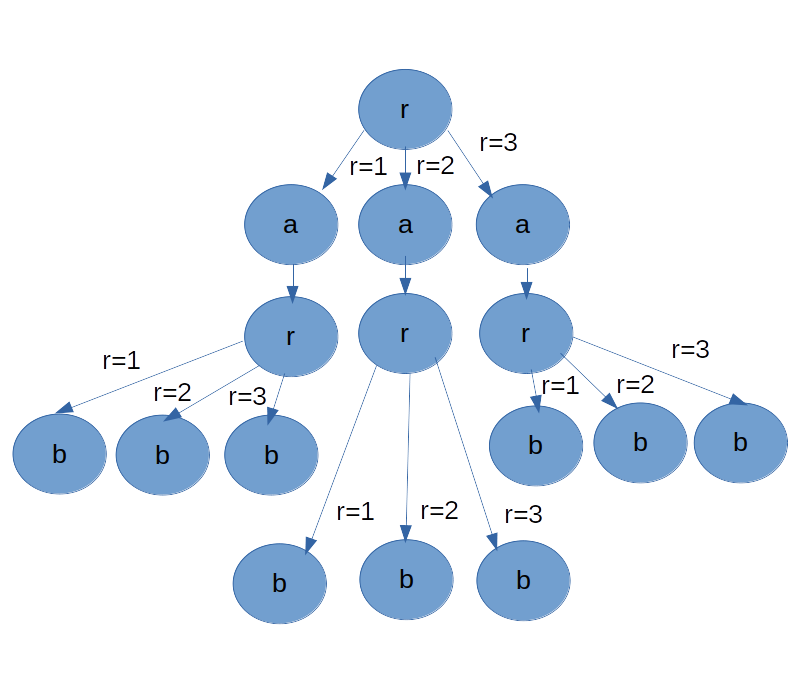
\includegraphics[width=0.9\linewidth]{Graphics/Neigh-Tree}
	\caption{Árbol de vecindad asociado a $rarb$}
	\label{fig:neigh-tree}
\end{figure}

Cada rama del árbol representa un conjunto de soluciones, por tanto, el conjunto de ramas representa una partición de la vecindad a la que está asociado dicho árbol. A los conjuntos hechos por esta partición se les denomina regiones y resultan útiles para encontrar características compartidas en grupos de vecindades. Por ejemplo, es conveniente analizar cuáles son las regiones con mejores soluciones para intensificar en estas la búsqueda de soluciones óptimas.

Luego de generadas las soluciones a partir del Árbol de Vecindad, es necesario conocer sus costos. Para esto se utiliza un Grafo de Evaluación.

\section{Grafo de Evaluación}\label{2-JJ}
Durante la exploración de las vecindades es (generalmente) necesario evaluar las soluciones que se van analizando. Ya sea para retornar inmediatamente una solución mejor a la inicial (estrategia de selección de primera mejora), para devolver la mejor solución (estrategia de selección de mejor vecino) o un vecino aleatorio entre todos los que mejoren la solución (estrategia de selección de mejor vecino aleatorio), en todos los casos hay que determinar el costo de las soluciones exploradas para analizar lo que es "mejor". Encontrar el costo de una solución es lo que se denomina como evaluar.

La evaluación de soluciones es potencialmente costosa. En el caso más simple se debe sumar las distancias entre cada cliente de cada ruta y el depósito. Agregar restricciones implica análisis extra como la aplicación de penalizaciones a rutas con vehículos sobrecargados en el caso de CVRP.

El Grafo de Evaluación, propuesto por Jose Jorge Rodríguez en \ref{2-JJ}, permite evaluar soluciones vecinas a una solución inicial de forma eficiente ya que garantiza que sólo se recalculan los fragmentos de las nuevas soluciones en los que estas se diferencien de la solución inicial.

La estructura propuesta es una representación en forma de grafo de la evaluación de la función objetivo en una determinada solución. Sus nodos están divididos en dos tipos: Nodos de alto nivel y nodos de bajo nivel. Los nodos de bajo nivel representan operaciones (incremento, decremento) que reciben como entradas ciertos nodos de alto nivel y modifican con sus salidas otros nodos de alto nivel.

Por ejemplo, en \ref{fig:eval-graph-1} se muestran los nodos de alto nivel del grafo que representa la solución:

\begin{equation}
s = [(c_1,c_2), (c_3,c_4)]
\end{equation}

Nótese que todas las rutas en el grafo comienzan y terminan con el nodo que representa al depósito. El nodo $cost$ almacena el valor del costo total de la solución.

\begin{figure}
	\centering
	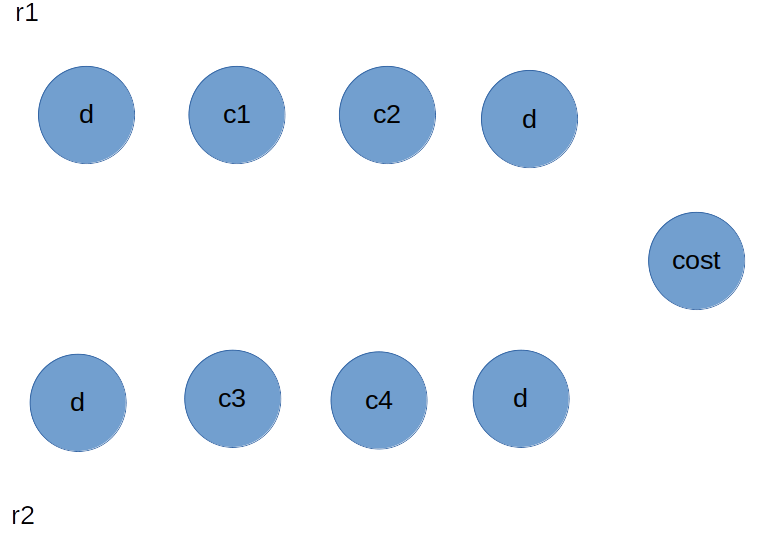
\includegraphics[width=0.9\linewidth]{Graphics/eval-graph-1}
	\caption{Nodos de alto nivel en un grafo de evaluación que representa la solución $s1$ de VRP clásico.}
	\label{fig:eval-graph-1}
\end{figure}

En \ref{fig:eval-graph-2} se muestra una representación del grafo completo para esta solución. Los nodos con símbolo de incremento son nodos de bajo nivel que toman como entrada dos nodos clientes (o depósito) y como salida adicionan al nodo de costo total la distancia entre ellos.

\begin{figure}
	\centering
	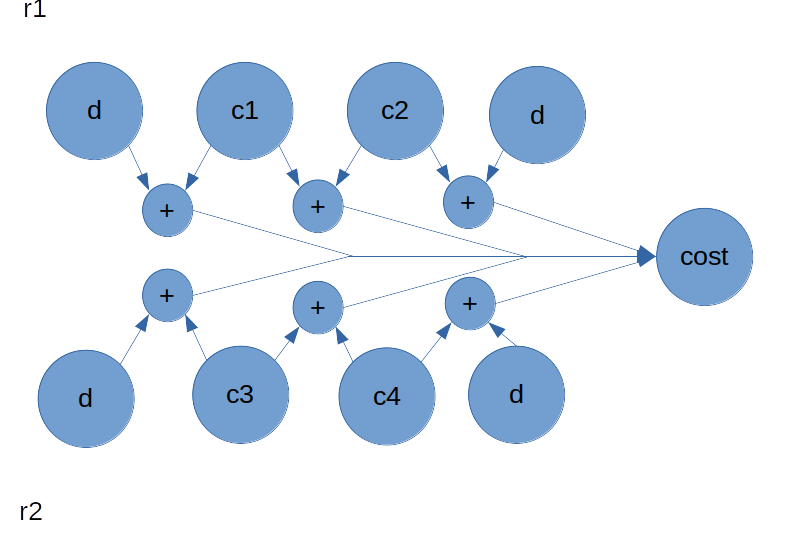
\includegraphics[width=0.9\linewidth]{Graphics/eval-graph-2}
	\caption{Grafo de evaluación que representa la solución $s1$ de VRP clásico.}
	\label{fig:eval-graph-2}
\end{figure}

En \ref{fig:eval-graph-3} se transforma el problema en CVRP utilizando la misma solución. En este caso se agregan los nodos de alto nivel $cap$ que tienen como valor inicial la capacidad del vehículo perteneciente a cada ruta. Los nodos de decremento reciben un cliente como entrada y, como salida, disminuyen la capacidad del vehículo en una cantidad igual a la demanda del cliente. Luego, los nodos $pen$ (también de bajo nivel) reciben como entrada los nodos de capacidad y, en caso de tener estos valor negativo, como salida penalizan el costo total de la solución.

 \begin{figure}
	\centering
	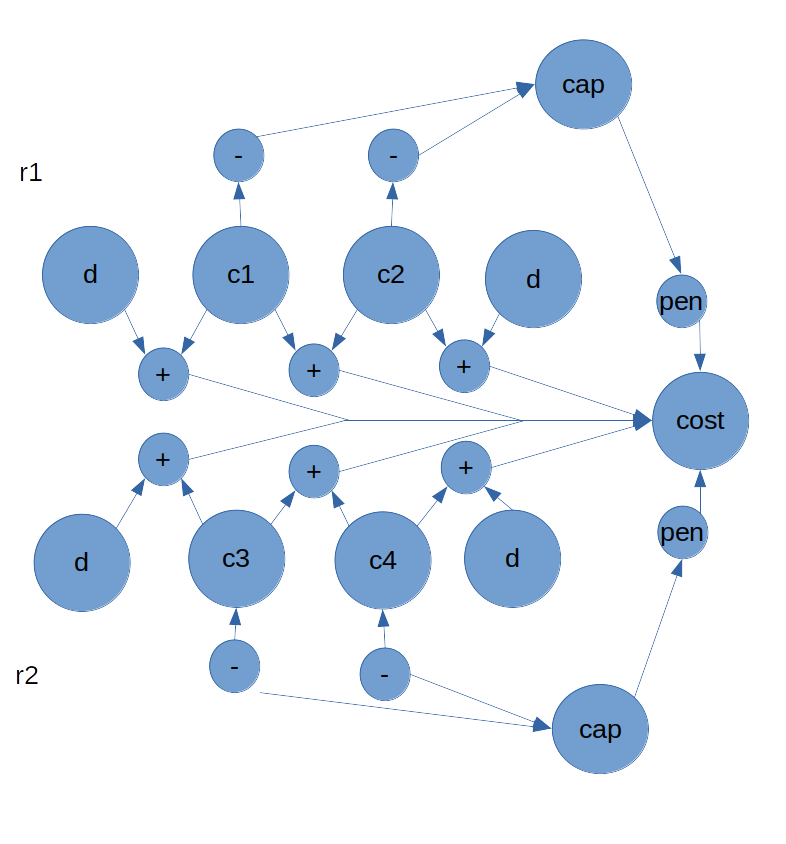
\includegraphics[width=0.9\linewidth]{Graphics/eval-graph-3}
	\caption{Grafo de evaluación que representa la solución $s1$ de VRP con restricciones de capacidad.}
	\label{fig:eval-graph-3}
\end{figure}

Todos los nodos de bajo nivel tienen asociado una función \textbf{evaluate} (para evaluar) y una función \textbf{undo} (para desevaluar) que son ejecutados cuando se agregan o remueven nodos de alto nivel. Por ejemplo, retirar un cliente $C1$ del grafo representado en \ref{fig:eval-graph-2} (VRP clásico) provoca que los dos nodos de incremento que utilizan dicho cliente como entrada se desevalúen y al mismo tiempo se crea un nuevo nodo incremento que recibe como entrada $d$ y $c2$. Luego, insertar a $c1$ al final de la ruta $r2$ implicaría desevaluar el nodo incremento que recibe como entrada a $c4$ y $d$ mientras se crean dos nodos incrementos nuevos, uno recibiendo de entrada a $c4$ y $c1$ mientras que el otro a $c1$ y $d$. El resultado de estas dos operaciones se muestra en \ref{fig:eval-graph-4} y es, precisamente, el grafo resultante de aplicar la siguiente instanciación del criterio $rarb$:

\begin{itemize}
	\item Seleccionar ruta (r1).
	\item Seleccionar cliente (c1) en ruta (r1).
	\item Seleccionar ruta (r2).
	\item Insertar cliente (c1) en posición (3) en ruta (r2).
\end{itemize}

Nótese que luego de aplicar los métodos \textbf{evaluate} y \textbf{undo} correspondientes el nodo $cost$ tiene almacenado el costo de la solución resultante luego de aplicar una instancia del criterio $rarb$. Para encontrar el costo de la nueva solución sólo fue necesario analizar y modificar los nodos en que el grafo de la solución nueva se diferencia con la solución anterior y no todo el grafo. En esto se basa la evaluación "eficiente" del Grafo de Evaluación.

 \begin{figure}
	\centering
	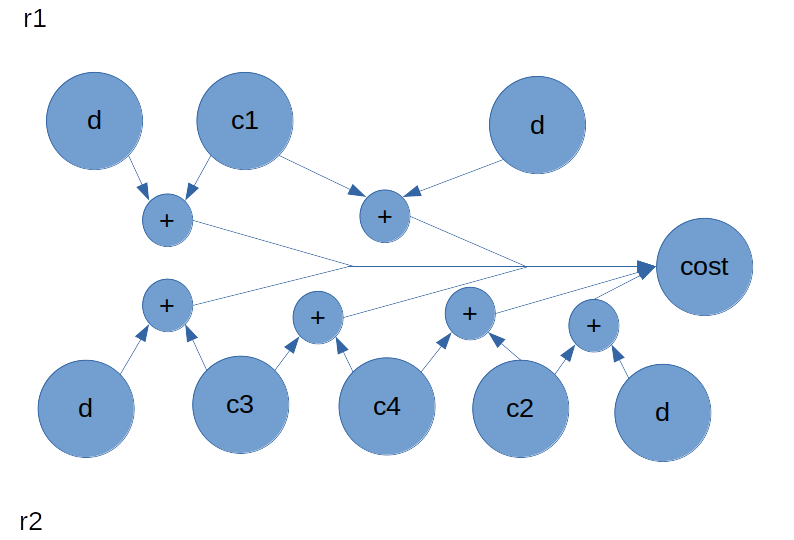
\includegraphics[width=0.9\linewidth]{Graphics/eval-graph-4}
	\caption{Grafo de evaluación que representa la solución $s1$ de VRP clásico luego de aplicada una instancia de $rarb$}
	\label{fig:eval-graph-4}
\end{figure}

Para construir el grafo que representa la solución inicial el usuario debe ingresar el códio de evaluación de esa primera solución. Luego, los costos el resto de las soluciones generadas son obtenidos al aplicar operaciones sobre el grafo inicializado.

Para explorar una vecindad a partir de un criterio es necesario (además de generar y evaluar soluciones) decidir e implementar estrategias de exploración y de selección. A partir de combinaciones de diferentes estrategias se pueden realizar montones de exploraciones distintas.


\section{Combinación de estrategias de exploración y selección.}\label{2-Heidy} 
En el proceso de exploración de una vecindad se parte de una solución inicial, se generan soluciones vecinas a esta (con el Árbol de vecindad) y se evalúan para comparar y obtener mejores soluciones (Grafo de Evaluación). Al explorar, deben también tenerse en cuenta problemas tales como la cardinalidad potencialmente enorme de los vecinos o el retorno de mínimos locales. Para una vecindad muy poblada tal vez dé mejor resultado explorar no todos sus vecinos, sino una porción aleatoria de estos. Tal vez retornar siempre al mejor vecino de cada vecindad pueda provocar el encuentro de un mínimo local que se hubiera evitado seleccionando aleatoriamente cualquier solución que mejorara la inicial.

Al espectro de búsqueda de vecinos en una vecindad se le denomina estrategia de exploración. Algunos ejemplos son:

\begin{itemize}
	\item Exploración exhaustiva: Se analizan todos los vecinos que puedan ser generados.
	\item Exploración aleatoria: Se genera una cantidad fija de vecinos menor que la cardinalidad de la vecindad. La decisión de qué vecinos generar es aleatoria.
\end{itemize}

Además de decidir qué vecinos explorar, también es necesario decidir cuál retornar entre aquellos que mejoran la solución. A esta decisión se le denomina estrategia de selección. Se tiene como ejemplos:

\begin{itemize}
	\item Mejor vecino: Se retorna al mejor vecino entre todos aquellos analizados.
	\item Primera mejora: En el momento en que se encuentra un vecino mejor que el inicial, este es retornado.
	\item Mejora aleatoria: Se retorna un vecino aleatorio entre todos aquellos mejores que la solución inicial.
\end{itemize}

A partir de distintas combinaciones de estrategias de exploración y selección es posible realizar numerosas exploraciones distintas que obtengan diferentes resultados.

La propuesta de Heidy Abreu en \cite{Heidy} permite generar funciones de exploración fabricadas a partir de un criterio, una estrategia de selección y una de exploración. Las estrategias se definen como clases que se pasan como instancias a la función generadora. La función resultante recibe el problema con una solución inicial, ejecuta la exploración y retorna una solución mejor en caso de existir dentro de la vecindad definida por el criterio. En este trabajo, el árbol de vecindad y el grafo de evaluación forman parte también de las funciones de exploración creadas. Un árbol de vecinad genera las soluciones y un grafo de evaluación de usa para evaluarlas. El grafo debe ser pasado como entrada.

La creación automática de funciones de exploración con distintas combinaciones de estrategias de exploración y selección se logra aprovechando sus características comunes y estructuras similares. El código generado en todas las funciones se reparte en cinco regiones que se  unen para generar una función completa. Las regiones y el tipo de código que pertenece a cada una se explicarán en \ref{TODO}.

El trabajo de generación de código y la creación de funciones a partir de estrategias diferentes se facilita mucho gracias a las características del lenguaje Common Lisp.

\section{Common Lisp y sus funcionalidades}\label{2-Lisp}
Common Lisp es un lenguaje de programación multi-paradigma (soporta una combinación de paradigmas de programación tales como la programación imperativa, funcional y orientada a objetos). Facilita el desarrollo de software evolutivo e incremental, con la compilación iterativa de programas eficientes en tiempo de ejecución.

El lenguaje acepta herencia múltiple. Esta característica permite crear jerarquías con clases que implementan funcionalidades de varias clases superiores. Por ejemplo, la clase que representa la estrategia de selección de mejor vecino (\textbf{best-improvement}) hereda de una clase que indica  retorno de mejor solución (\textbf{return-best-solution}) y de otra que indica el uso de un grafo de evaluación (\textbf{use-eval-graph}).

La herencia útil resulta especialmente útil para el presente trabajo cuando se combina con el sistema CLOS (Common Lisp Object System). Un mismo método puede tener numerosas implementaciones (especificaciones) que se ejecutan de acuerdo a los tipos de los parámetros proveídos como entradas. Además, también se ejecutan todas las especificaciones cuyos parámetros coincidan con los ancestros de los tipos de las entradas. Todas las especificaciones se combinan alrededor de un método primario conformando un único método con la unión de todos los códigos. El orden en que se combinan los métodos depende del orden de herencia y de los parámetros :before, :around y :after con que se definen.

Como ejemplo se tiene que para generar el código de la función de exploración para la estrategia de selección de menor vecino se une el código de métodos cuyo parámetro de \text{search-strategy} tenga tipo \textbf{best-improvement}, \textbf{return-best-solution}, \textbf{use-eval-graph} y cualquier otra clase que herede de alguna de estas.




























\chapter{Propuesta de solución}\label{chapter:Solution}

En este capítulo se ofrece la estructura general que representa la solución propuesta para codificar soluciones del VRP a un espacio continuo. Su diseño abstracto mediante dos componentes principales, \textit{encoder} y \textit{decoder}, permite la rápida adaptación de otra arquitectura de redes neuronales al modelo general. 

Como parte de la implementación se formularon dos modelos concretos para resolver el problema de codificación, \textit{\textbf{LinearAEC}} y \textit{\textbf{VAE}}. El primero de ellos está basado en un modelo \textit{autoencoder} clásico y el segundo, en un \textit{variational autoencoder}.

También se describe la etapa de generación y procesamiento de los datos para conformar los conjuntos de entrenamiento, prueba y validación. En este punto se retoman los tipos de representación vectorial de soluciones del VRP expuestos en la sección \ref{2-solS}.

A continuación se explica la idea central del problema, el procesamiento de los datos y el diseño de la solución. 


\section{Definición del problema}

La codificación de soluciones del VRP de un espacio discreto a vectores reales, surge por el interés de investigar el espacio continuo que puede obtenerse con el empleo de un modelo \textit{autoencoders} a partir de soluciones discretas del VRP.
De ahí que sea fundamental lograr una representación continua capaz de capturar sus características y propiedades.

El VRP es un problema de optimización combinatoria cuyo objetivo es minimizar el
 valor de una función de costo $C$ sobre el espacio $\mathcal{S}$ de soluciones, es decir $min \; C(s), \: s\in \mathcal{S}$ teniendo en cuenta las características y restricciones del problema. El espacio $\mathcal{S}$ lo forman soluciones representadas por vectores discretos, bien podrían ser cualquiera de las representaciones vistas en el capítulo \ref{chapter:REV-LL}. En este caso se considera que $\mathcal{S} \subset \mathbb{R}^{n}$, está formado por vectores con la misma estructura que los vectores $p$ analizados en \ref{2-Graph}.
 
 
 %En este caso $\mathcal{S}$ constituye un espacio de soluciones discretas del VRP, bien  y $\mathcal{S} \subset \mathbb{R}^{t}$ para algún $t$.
 
 La intención de este trabajo es obtener una representación $z \in \mathcal{Z}$ a partir de $s$, donde $\mathcal{Z}$ es un espacio continuo $\mathcal{Z} \subset \mathbb{R}^{l}$, para algún $l$. Es decir, determinar una función:
 \begin{equation}
 	f: \mathcal{S} \rightarrow \mathcal{Z},
 \end{equation}
 de forma tal que $f(s) = z$, y además, recuperar la solución codificada en $z$ mediante otra función:
  \begin{equation}
  g: \mathcal{Z} \rightarrow \mathcal{S},
  \end{equation}
 cuyo objetivo es conseguir que el resultado de $g(z) = s'$ sea lo más cercano posible a la entrada original $s$. Con esta idea, las soluciones iniciales $s$ se podrán representar mediante vectores con valores reales cuya dimensión depende de la dimensión del problema, y se conoce como código, vector de contexto o vector latente. 
 
Sea $s$ una solución del VRP, el problema enunciado puede reducirse a aproximar las funciones $f$ y $g$ de forma tal que $f(s) = z$ y $g(z) = s$ con el uso de técnicas de aprendizaje profundo, en particular: modelos \textit{autoencoders}. La funciones $f$ y $g$ se denominan \textit{encoder} y \textit{decoder} respectivamente y están constituidas por redes neuronales. La arquitectura específica del modelo se precisará en la sección \ref{3-GenStruct}, pero antes se describe el proceso seguido para generar los datos empleados en el proceso de entrenamiento.


\section{Procesamiento de datos de entrenamiento}\label{dataProc}

Una cuestión importante que se debe abordar antes de introducir el modelo es el procesamiento y preparación de los datos de entrada tal y como se señaló en \ref{1-etapas}. Como parte de esta etapa, se pueden aplicar varias técnicas que dependen del tipo de datos con los que se cuenta, por ejemplo si son de tipo texto o imagen. 

%En este caso se parte de la generación de soluciones del VRP representadas mediante los vectores $p$ explicados en \ref{2-Graph}, que luego se convierten a matrices 

El procesamiento previo permite una mejor adaptación entre los datos y la red neuronal mediante una serie de técnicas como vectorización de la información y normalización. Considerando que en la representación vectorial expuesta en \ref{2-Graph} con los vectores $p$, los valores no están normalizados, se decidió representar los datos a través de las matrices binarias $M$ analizadas en \ref{2-Matrix}. 

Como el objetivo principal es la codificación de una solución a un vector real, solo interesan en ellas, los clientes y cantidad $m$ de rutas. La conformación del conjunto de datos o soluciones iniciales para una instancia particular con $n$ clientes se desarrolló generando los vectores $p$, que como se había explicado, establecen la adyacencia en el grafo formado a partir de las rutas contenidas en la solución. Una vez obtenido ese conjunto de datos, cada solución del mismo se convierte a la matriz $M$ correspondiente, con el fin de obtener una representación normalizada.   

%Teniendo en cuenta las definiciones \ref{2-pi} y \ref{2-Matrix}, correspondientes a los vectores $p$ y las matrices binarias $M$ respectivamente, la transformación de un vector $p$ a una matriz $M$ se establece como sigue:


%Una instancia de un problema de enrutamiento de vehículos está definida por la cantidad de clientes $n$ y la cantidad de vehículos $m$. La conformación inicial del conjunto de datos para una instancia particular se desarrolló generando vectores $p$ que constituyen planificaciones de $m$ rutas para satisfacer los $n$ clientes. Luego de ello, se realiza una transformación sobre cada vector generado para obtener una  representación normalizada con matrices binarias.

%Sea $s \in \mathcal{S}$ una solución discreta a una instancia del VRP con $n$ clientes y $m$ vehículos, $p$ el vector de dimensión $n$ correspondiente según la interpretación ofrecida con grafos dirigidos, y $M$ la matriz binaria que se obtiene a partir de $p$. Primeramente se retoma la definición de ambas representaciones vectoriales:

%\[p[j]=\left\{
%\begin{array}{rcl}
%i & \mbox{si} & \text{el cliente $j + 1$ va detrás de $i + 1$ en la ruta. }\\
%&
%& \\
%j & \mbox{si} & \text{el cliente $j + 1$ es comienzo de ruta. }  \\
%&
%& \\
%\end{array}
%\right. \]


%\[M[i, j]=\left\{
%\begin{array}{rcl}
%1 & \mbox{si} & \text{el cliente $j + 1$ va detrás de $i + 1$ en la ruta.}\\
%&
%& \\
%1 & \mbox{si} & \text{$i = j$, la ruta está formada por un único cliente i + 1.}  \\
%&
%& \\
%0 & \mbox{eoc}  \\
%\end{array}
%\right. \]


%\[M[i, j]=\left\{
%\begin{array}{rcl}
%\label{Pi2M}
%1 & \mbox{si} & \text{$p[j] = i, \; i \neq j$}\\
%&
%& \\
%1 & \mbox{si} & \text{$p[j] = j, \; j + 1$ es el único cliente en su ruta}  \\
%&
%& \\
%0 & \mbox{eoc}  \\
%\end{array}
%\right. \]

%A continuación se muestra el procedimiento seguido para obtener $M$ a partir de $p$ mediante un ejemplo concreto. En particular se considerá el mismo vector de 9 clientes analizado en \ref{2-Graph}:
%\begin{center}
%	$p = [4, 1, 7, 5, 1, 5, 6, 6, 8],$
%\end{center}
%que se corresponde con la solución a través de listas de rutas:
%\begin{center}
%	$s = [(2, 5, 1), (6, 4), (7, 8, 3), (9)].$
%\end{center}

%Finalmente los pasos realizados se resumen en:
%\begin{eqnarray*}
%	p[0] = 4 \rightarrow  M[4, 0] = 1,\\
%	p[2] = 7 \rightarrow  M[7, 2] = 1,\\
%	p[3] = 5 \rightarrow  M[5, 3] = 1,\\
%	p[4] = 1 \rightarrow  M[1, 4] = 1,\\
%	p[7] = 6 \rightarrow  M[6, 7] = 1,\\
%	p[8] = 8 \rightarrow  M[8, 8] = 1, 
%\end{eqnarray*}

%El resto de las posiciones de $M$ tomarán valor 0 según la tercera condición de \ref{Pi2M}. Finalmente la matriz resultante es:

 %\begin{equation}
%\centering
%\begin{pmatrix}
%0 & 0 & 0 & 0 & 0 & 0 & 0 & 0 & 0\\
%0 & 0 & 0 & 0 & 1 & 0 & 0 & 0 & 0\\
%0 & 0 & 0 & 0 & 0 & 0 & 0 & 0 & 0\\
%0 & 0 & 0 & 0 & 0 & 0 & 0 & 0 & 0\\
%1 & 0 & 0 & 0 & 0 & 0 & 0 & 0 & 0\\
%0 & 0 & 0 & 1 & 0 & 0 & 0 & 0 & 0\\
%0 & 0 & 0 & 0 & 0 & 0 & 0 & 1 & 0\\
%0 & 0 & 1 & 0 & 0 & 0 & 0 & 0 & 0\\
%0 & 0 & 0 & 0 & 0 & 0 & 0 & 0 & 1\\
%\end{pmatrix}
%\end{equation}
%la cual coincide con la misma analizada en \ref{M9}.

%Dada la estructura y propiedades de este tipo de matrices, es fácil revertirlas para obtener la solución $s$ correspondiente. No obstante, como no se establece una biyección entre $s$ y $M$, la generación de los datos será mediante otro array que se nombrará como $pi$. 

Una vez representadas las soluciones del VRP como un vector donde cada componente pertenece al intervalo $[0, 1]$, se puede presentar la estructura general del modelo propuesto en la siguiente sección.

%Como se había mencionado, la solución implementada posee una estructura general a la cual se adaptaron los dos modelos propuestos, específicamente, evidenciada en el uso de sus dos componentes principales. En la siguiente sección se profundiza sobre esta cuestión. 


\section{Estructura general del modelo propuesto}\label{3-GenStruct}

El modelo ofrecido en este trabajo para la codificación de soluciones de un problema VRP, sigue la idea general de los modelos \textit{autoencoders} descritos en \ref{2-AEC} y consiste en dos componentes principales:  \textit{encoder} y \textit{decoder}. En la figura \ref{modelGeneral} se muestra un esquema general del modelo.

\begin{figure}[!h]
	\centering
	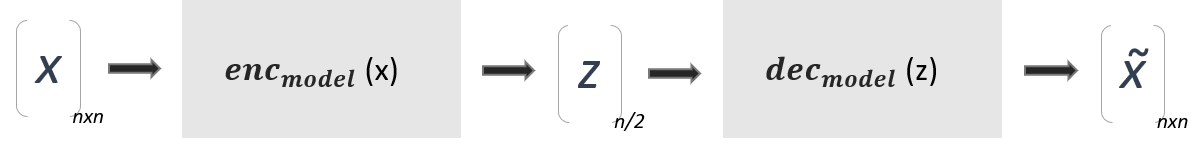
\includegraphics[width=5in]{Graphics/model general.png}
	
	\caption{ \small{Esquema general del modelo propuesto con las componentes \textit{encoder} y \textit{decoder}.}}
	
	\label{modelGeneral}
\end{figure}  

Dichas componentes son las encargadas de aproximar las funciones $f$ y $g$ mencionadas en la definición del problema, de foma tal que $f$ se reemplaza por la componente \textit{encoder} y $g$ se sustituye por la componente \textit{decoder}. Ambas están relacionadas mediante tres vectores que juegan un papel fundamental: el vector de entrada $x$, vector de contexto $z$ y el vector de salida $\tilde{x}$.

Los \textbf{vectores de entrada} constituyen matrices binarias de dimensión $n \times n$ representando a las soluciones del VRP. Además de ser la entrada a la red general, son la entrada de la componente \textit{encoder}. Este devuelve como salida un vector real denotado por $z$ que se conoce como \textbf{vector de contexto}. Posteriormente el \textit{decoder} procesa el vector $z$ y retorna un \textbf{vector de salida} que establece una reconstrucción de la entrada $s$. Tanto la entrada inicial al modelo como la salida final presentan las mismas dimensiones como se observa en el esquema \ref{modelGeneral}.

La configuración de parámetros en las componentes y la dimensión del vector $z$ dependen de la dimensión del problema, por tanto, la arquitectura del modelo se ajusta al tipo de problema particular. Debido a ello es necesario entrenar el modelo para cada dimensión del problema, o sea, para una cantidad de clientes fija.


\subsection{Funcionalidades del modelo propuesto}

La estructura genérica presentada anteriormente permite el uso de las componentes \textit{encoder} y \textit{decoder} de forma independiente, una vez que se entrene el modelo. En este sentido se distinguen tres funcionalidades que cumple el esquema general de la solución.

Siguiendo las definiciones señaladas en este capítulo, se denotará como $s$ el vector de entrada al modelo que representa una solución del VRP, $z$ el vector de contexto representativo de $s$ en el espacio continuo y $s'$ la reconstrucción de $s$ y también salida del modelo. A partir de este momento, las componentes \textit{encoder} y \textit{decoder} también serán tratadas como $enc_{model}$ y $dec_{model}$. 

Las funcionalidades referidas se exponen a continuación:

\begin{itemize}
	\item \textbf{codificar (encode)}: Mediante esta función es posible obtener el vector de código para una entrada $s$ cualquiera, de forma tal que:
	\begin{equation}
		encode(s) = enc_{model}(s) = z
	\end{equation}
	\item \textbf{decodificar (decode)}: A partir de un vector $z$ del espacio continuo, se puede producir la solución correspondiente en el espacio discreto aplicando:
	\begin{equation}
	decode(z) = dec_{model}(z) = s'
	\end{equation}
	
	\item \textbf{predecir (predict)}: Esta función da como resultado el vector reconstruido luego de atravesar por las dos etapas básicas de codificación y decodificación. Su empleo tiene sentido con el modelo ya entrenado para comprobar el desempeño del mismo. El funcionamiento consiste en:
	\begin{equation}
	predict(s) = dec_{model}(enc_{model}(s)) = s'
	\end{equation}
\end{itemize}

En la siguiente sección se profundizará en la descripción de ambos modelos, teniendo en cuenta la arquitectura de redes neuronales seleccionada.


\section{Modelos propuestos}

Como parte de la implementación de la propuesta de solución, se diseñaron dos modelos \textit{autoencoders} para intentar resolver el problema: \textit{\textbf{LinearAEC}} y \textit{\textbf{VAE}}. El primero de ellos conformado sobre la base de un \textit{autoencoders} clásico y el segundo, como su nombre lo indica, ideado a partir de un prototipo de VAE tradicional.

La función de pérdida de reconstrucción empleada en ambos modelos fue $MSE$ (Mean Squared Error), el promedio del cuadrado de las diferencias entre la entrada y la salida. La última capa de cada modelo utiliza la función de activación \textit{sigmoid}, y además, se decidió usar como optimizador \textit{RMSProp}, siguiendo las sugerencias brindadas en \textit{Chollet et al.} \cite{Chollet}. En el resto de las capas de ambos, se utiliza la función de activación \textit{relu}.

En lo adelante se denotarán como $E_i$ y $D_i$ las capas pertenecientes a las redes \textit{encoder} y \textit{decoder} respectivamente. Las características específicas, arquitectura y configuración de ambas propuestas serán abordadas en las siguientes secciones.
 

\subsection{Modelo \textit{LinearAEC}}\label{LinearAEC}

El carácter lineal de esta propuesta está determinado por la arquitectura de capas densas empleado. Tal y como se mencionó en \ref{3-GenStruct}, se encuentra conformado por dos componentes principales y tres vectores importantes. La configuración de la arquitectura y los parámetros correspondientes será detallada a continuación.

\subsubsection{Arquitectura del modelo}

Ambas componentes principales \textit{encoder} y \textit{decoder} constituyen redes neuronales formadas por capas densas. En la figura \ref{AECmodel} se muestra la estructura interna del modelo de inicio a fin:\\

\newpage

\begin{figure}[!h]
\centering
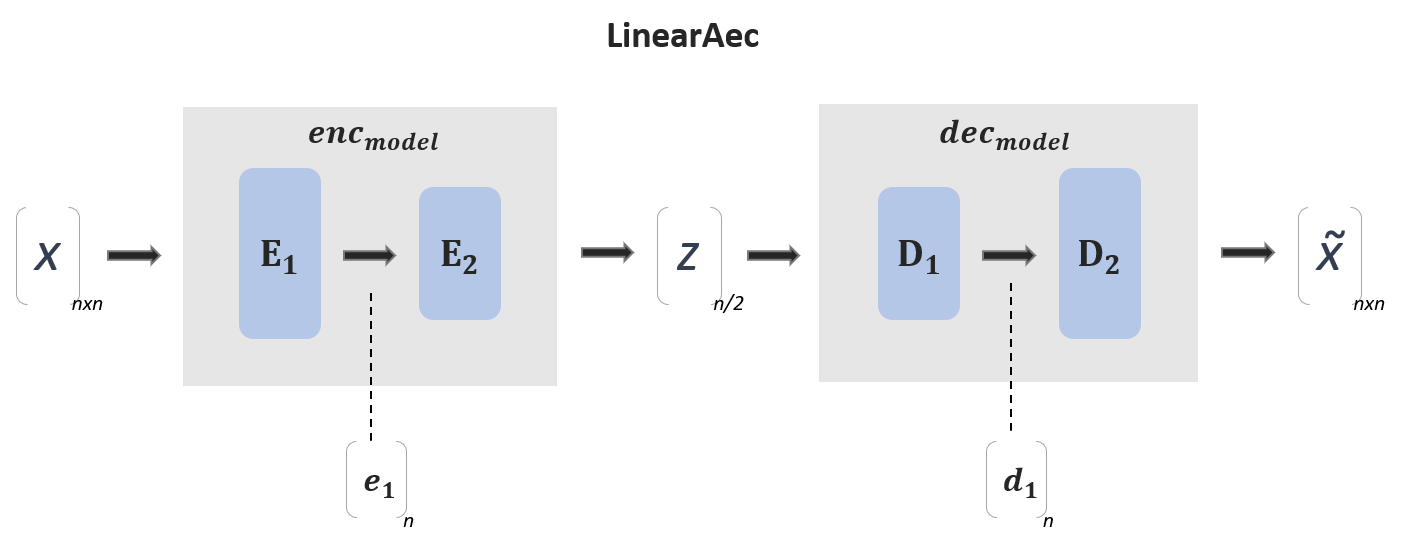
\includegraphics[width=5in]{Graphics/Aecmodel.png}

\caption{ \small{Diagrama del modelo LinearAEC}}

\label{AECmodel}
\end{figure}  


El \textit{encoder} recibe una matriz de entrada $x$ la cual se introduce a la primera capa oculta $E_1$. La salida de esta se conforma mediante la función de activación \textit{relu} y pasa a ser la entrada de la siguiente capa $E_2$, encargada de devolver el vector de contexto $z$. Durante la codificación, la dimensión de los vectores entre una capa y otra va disminuyendo hasta obtener $z$.

Posteriormente, $z$ se convierte en la entrada de la red \textit{decoder} donde será decodificado con el objetivo de recuperar la entrada $x$ inicial. La primera capa de entrada $D_1$ en esta componente, recibe el vector latente y devuelve como salida un vector de mayor dimensión con respecto a $z$, que será la entrada de la última capa $D_2$. Esta capa es la encargada de reconstruir la solución representada en $x$. Durante el proceso de decodificación la dimensión de los vectores de salida va incrementando en correspondencia con la disminución que se establece con la codificación. Por tal motivo, se puede decir que ambos procesos sin simétricos.





\subsection{Modelo \textit{VAE}}
Los VAE constituyen una versión más moderna de los \textit{autoencoders} que proporcionan una noción probabilística para describir un punto del espacio latente. En lugar de generar valores directamente para el estado latente como se hace en \ref{LinearAEC}, el modelo de codificación de un VAE generará parámetros que describen un distribución para cada dimensión en el espacio latente. Dado que se asume una distribución Normal, se generan dos vectores que describen la media y varianza de las distribuciones del espacio. Al generar puntos de tal distribución se obtienen nuevos datos, por eso es considerado un modelo generativo. Finalmente el \textit{decoder} procederá a desarrollar una reconstrucción de la entrada original. 

\subsubsection{Arquitectura del modelo} 


Similar al \textit{LinearAEC}, en el \textit{VAE}, las componentes \textit{encoder} y \textit{decoder} constituyen redes neuronales conformadas por capas densas. Lo interesante y diferente en este modelo, con respecto al \textit{LinearAEC}, es el proceso intermedio donde se genera el vector latente $z$. En la figura \ref{VAEmodel} se muestra un diagrama de la estructura interna del \textit{VAE} implementado, que facilitará la comprensión de sus etapas.\\


\begin{figure}[!h]
	\centering
	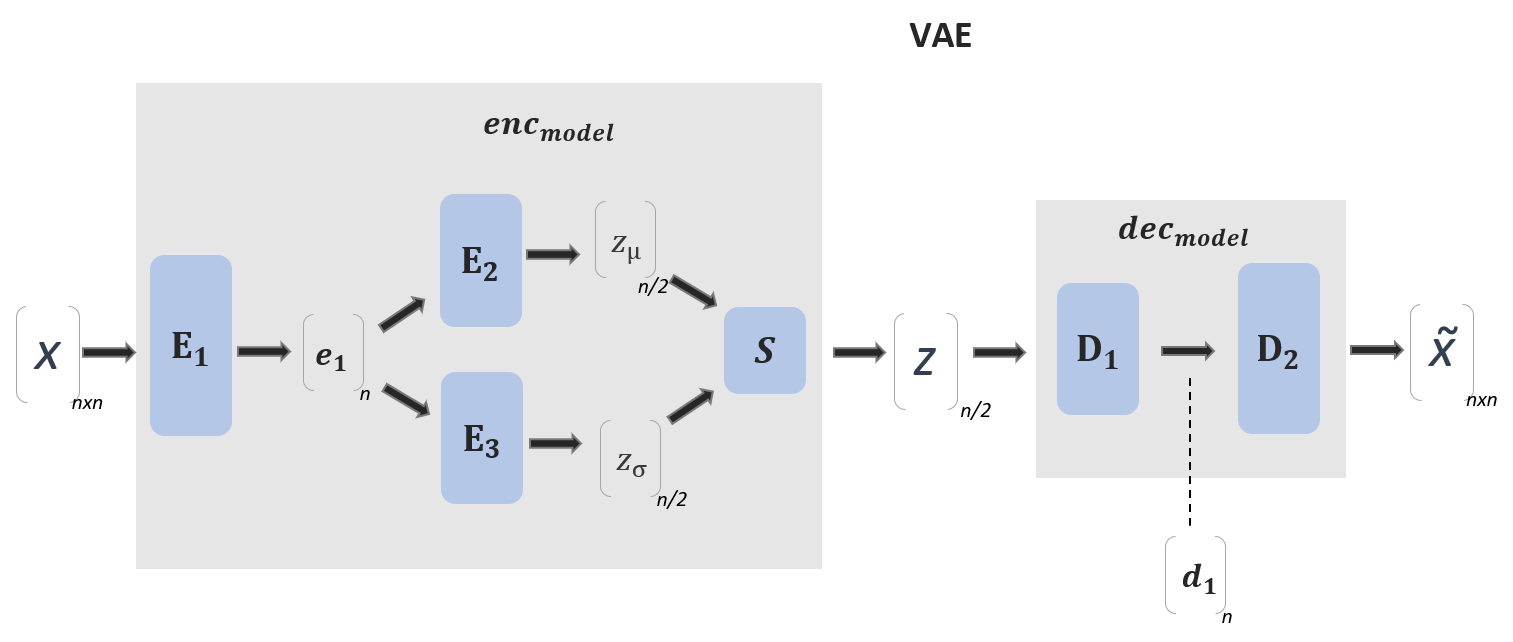
\includegraphics[width=5in]{Graphics/vaemodel.png}
	
	\caption{ \small{Diagrama del modelo VAE}}
	
	\label{VAEmodel}
\end{figure}  

El \textit{encoder} recibe un vector de entrada $x$ de dimensión $nxn$ el cual se procesa por la  capa de entrada $E_1$. A partir de este punto, es donde el proceso de codificación cambia en comparación con el \textit{LinearAEC}. Pues la salida de $E_1$ se introduce paralelamente a otras dos capas ocultas independientes que se identifican como $E_2$ y $E_3$.

El papel de estas nuevas capas es producir los vectores que describen la distribución de las codificaciones $z$. A través de $E_2$ se obtiene $z_{mean}$ y con $E_3$ se origina $z_{log {\_} sigma}$. Hasta el momento se ha explicado el punto número 1 de \ref{VAESteps}, donde se tiene que:

\begin{equation}
	z_{mean} , \; z_{log\_sigma} = enc_{model}(x)
\end{equation} 

Como parte de la generación del vector $z$ con los parámetros de la media y varianza de la distribución, se creó una capa personalizada que se denomina \textit{Sampling}. La capa se denota como $S$ en la figura \ref{VAEmodel}, recibe los parámetros mencionados y su esencia consiste en $	z = z_{mean} + exp(z_{log{\_}sigma})*\epsilon$. 

Una vez generado el vector $z$, este se convierte en la entrada del \textit{decoder}. En lo adelante, el comportamiento del \textit{decoder} es igual a la decodificación en el \text{LinearAEC}. Constituido por dos capas densas consecutivas $D_1$ y $D_2$, donde el vector de salida va aumentando de dimensión de una capa a la otra. Finalmente se obtiene la salida $\tilde{x}$ como reconstrucción de la entrada inicial $x$.\\

En el presente capítulo se expusieron dos modelos concretos para obtener una representación continua de las soluciones del VRP. Ambos se sustentan en la teoría analizada en el capítulo \ref{chapter:REV-LL} e intentan describir una distribución de probabilidad de los vectores de codificación. En el siguiente capítulo se muestran los resultados obtenidos a partir de dos escenarios donde se evalúa el comportamiento de los mismos.



 




\chapter{Método de uso}\label{chapter:Tutorial}

Este capítulo explica los pasos que debe seguir un usuario para resolver variantes de VRP utilizando el sistema que se implementó en este trabajo. Esto se hará a través de un ejemplo de resolución de un problema CVRP arbitrario.

En la sección \ref{4-problem} se define el problema. En la sección \ref{4-solution} se construye el grafo de evaluación y la solución inicial. En la sección \ref{4-generator} se generan las funciones de exploración. En \ref{4-union} se presenta el código completo.

\section{Definición del problema}\label{4-problem}

El primer paso para resolver un VRP usando este sistema, es definirlo usando las clases que lo representan a él y a sus características. Esto se mostrará a través de un ejemplo de resolución de un CVRP con seis clientes. En este caso, se debe crear un objeto de tipo \texttt{basic-cvrp-client} (cliente con demanda) por cada cliente, uno de tipo \texttt{basic-depot} (depósito) y una matriz de distancias de tamaño $6x6$. 

El siguiente código se usa para definir el problema.

 \begin{lstlisting}
(defparameter c1 (basic-cvrp-client 1 1))
(defparameter c2 (basic-cvrp-client 2 1))
(defparameter c3 (basic-cvrp-client 3 4))
(defparameter c4 (basic-cvrp-client 4 3))
(defparameter c5 (basic-cvrp-client 5 2))
(defparameter c6 (basic-cvrp-client 6 1))

(defparameter d0 (basic-depot))

(defparameter dist-mat #2A((0 1 2 3 4 5 6)
										(1 0 5 2 1 3 2)
										(2 5 0 2 2 2 2)
										(3 2 2 0 1 2 1)
										(4 1 2 1 0 2 3)
										(5 3 2 2 2 0 1)
										(6 2 2 1 3 1 0)))

(defparameter problem (basic-cvrp-problem 
										:id 1 
										:clients (list c1 c2 c3 c4 c5 c6)
										:depot d0 
										:distance-matrix dist-mat 
										:capacity 20))
\end{lstlisting}

En las líneas 1 a 6 se definen los clientes, estos reciben dos parámetros, \textit{id} y \textit{demanda} respectivamente. Los vehículos se definen en las líneas 8 y 9, reciben también dos parámetros \textit{id} y \textit{capacidad} respectivamente. Luego se declara el depósito (línea 11), la matriz de distancias (línea 13) y se crea la instancia del problema (línea 21).

Una vez se definió el problema, se debe crear una solución inicial como se muestra en la siguiente sección.

\section{Solución inicial y Grafo de Evaluación}\label{4-solution}

La solución inicial se utiliza para construir e inicializar el grafo. En el caso de CVRP una solución está formada por una lista de rutas que son instancias de la clase \texttt{route-for-simulation}. El siguiente código muestra cómo se crea una solución:


\begin{lstlisting}
(defparameter r1 (route-for-simulation 
							:id 1
							:vehicle (cvrp-vehicle 1 20) 
							:depot d0
							:clients (list c1 c2 c3 (clone d0))
							:previous-client (clone d0)))
(defparameter r2 (route-for-simulation 
							:id 2 
							:vehicle (cvrp-vehicle 2 20)
							:depot d0
							:clients (list c4 c5 c6 (clone d0))
							:previous-client (clone d0)))

(defparameter s1 (basic-solution
							:id 1 
							:routes (list r1 r2)))
\end{lstlisting}

Las rutas se definen como instancias de la clase \texttt{rute-for-simulation} (líneas 1 y 7). Esta clase hereda de la clase \texttt{basic-route} y la extiende con la propiedad \textit{previous-client}. Esta propiedad se inicializa con una referencia al depósito a partir de la cual se crea el primer nodo de la ruta en el grafo de evaluación y simplifica la implementación del código de evaluación de la solución. Nótese que las rutas del grafo de evaluación comienzan y terminan en el depósito que se debe clonar para tener, en cada posición, nodos distintos.

Luego se debe inicializar el grafo con la función \texttt{init-graph}.

\begin{lstlisting}
(defparameter graph (init-graph s1))
\end{lstlisting}

Una vez que el grafo está inicializado, se le deben agregar las operaciones y nodos que mantienen valores. Esto se consigue mediante el código de evaluación de la solución inicial.

\begin{lstlisting}
(def-var total-distance 0 graph)
(loop for r in (routes s1) do
	(def-var route-distance 0 graph)
	(def-var route-demand (capacity (vehicle r)) graph) 
	(loop for c in (clients r) do 
		(increment-distance (previous-client r) c route-distance dist-mat graph)
		(decrement-demand c route-demand graph) 
		(setf (previous-client r) c)
	(increment-value total-distance route-distance graph)
	(apply-penalty route-demand total-distance 10 graph)
(return-value total-distance graph))
\end{lstlisting}

En la línea 1 se usa \texttt{def-var} para inicializar la variable que almacena el costo total de la solución. Luego se analizan las rutas de la solución. Por cada ruta se define una variable nueva que almacena su costo (línea 3) y otra que almacena la capacidad restante de su vehículo (línea 4). Entonces se analizan los clientes de la ruta actual. Se incrementa el costo de la ruta en una cantidad igual a la distancia del cliente actual y el cliente previo (el cliente previo inicial de la ruta es el depósito), y se disminuye la capacidad del vehículo en una cantidad igual a la demanda del cliente (líneas 6 y 7 respectivamente). Después de analizar cada ruta se aumenta el costo total de la solución en una cantidad igual a los costos de las mismas y se aplica penalización en caso de que un vehículo haya alcanzado una capacidad restante negativa (líneas 9 y 10). Finalmente se retorna la distancia total.

La siguiente sección ejemplifica cómo se generan las funciones de exploración a partir de criterios de vecindad y estrategias de exploración y selección.

\section{Generación de funciones de exploración}\label{4-generator}

Una vez que se tiene el grafo de evaluación de una solución inicial, para resolver el problema con una búsqueda local se debe definir cómo explorar la vecindad.

Las estrategias de exploración y selección se definen como clases cuyas instancias se pasan como parámetros a la función generadora. Se utilizan métodos que reciben estas instancias y generan código a partir de especializaciones de los tipos de los argumentos recibidos.

A continuación se presentan algunas clases que representan estrategias de exploración y selección:\\

\textit{Exploración:}
\begin{itemize}
	\item \texttt{exhaustive-neighborhood-search-strategy}: Exploración exhaustiva.
	\item \texttt{random-neighborhood-search-strategy}: Exploración aleatoria.
\end{itemize}

\textit{Selección:}
\begin{itemize}
	\item \texttt{best-improvement-search-strategy}: Selección de mejor solución.
	\item \texttt{first-improvement-search-strategy}: Selección de primera mejora.
	\item \texttt{random-improvement-with-candidates-selection-strategy}: Selección aleatoria de una mejora entre los elementos de una lista con las mejoras encontradas.
	\item \texttt{random-improvement-selection-strategy}: Selección aleatoria de una mejora en base a una probabilidad.
\end{itemize}

Durante la definición de cada clase se crea un parámetro global que almacena una instancia de su respectiva clase. Por ejemplo, el parámetro \texttt{+exhaustive-search-strategy+} tiene como valor asociado una instancia de \texttt{exhaustive-neighborhood-search-strategy}.

A continuación se define una lista de funciones de exploración para los criterios \textit{mover un cliente dentro de su ruta}, \textit{mover un cliente a cualquier ruta en cualquier posición} e \textit{intercambiar dos clientes de posición}. En todos los casos se hace una búsqueda exhaustiva con selección de mejor vecino.

\begin{lstlisting}
(setf rab (make-neighborhood-criterion 
						`((select-route r1)
						(select-client c1 from r1)
						(insert-client c1 to r1))
						+exhaustive-search-strategy+ 
						+best-improvement+))

(setf rarb (make-neighborhood-criterion 
						`((select-route r1)
						(select-client c1 from r1)
						(select-route r2)
						(insert-client c1 to r2))
						+exhaustive-search-strategy+ 
						+best-improvement+))

(setf rarac (make-neighborhood-criterion 
						`((select-route r1)
						(select-client c1 from r1)
						(select-route r2)
						(select-client c2 from r2)
						(swap-clients c1 c2))
						+exhaustive-search-strategy+ 
						+best-improvement+))

(setf criteria (list rab rarb rarac))

\end{lstlisting}

En este punto es posible invocar la función de metaheurística de Búsqueda de Vecindad Variable y obtener una solución.

\begin{lstlisting}
(setf result (vns-vrp-system problem criteria graph :max-iter 1000))
\end{lstlisting}

La siguiente sección muestra el código completo que soluciona un CVRP con datos ficticios.

\section{Código completo}\label{4-union}

\begin{lstlisting}
(defparameter c1 (basic-cvrp-client 1 1))
(defparameter c2 (basic-cvrp-client 2 1))
(defparameter c3 (basic-cvrp-client 3 4))
(defparameter c4 (basic-cvrp-client 4 3))
(defparameter c5 (basic-cvrp-client 5 2))
(defparameter c6 (basic-cvrp-client 6 1))


(defparameter d0 (basic-depot))

(defparameter dist-mat #2A((0 1 2 3 4 5 6)
										(1 0 5 2 1 3 2)
										(2 5 0 2 2 2 2)
										(3 2 2 0 1 2 1)
										(4 1 2 1 0 2 3)
										(5 3 2 2 2 0 1)
										(6 2 2 1 3 1 0)))

(defparameter problem (finite-fleet-cvrp-problem 
										:id 1 
										:clients (list c1 c2 c3 c4 c5 c6)
										:depot d0 
										:distance-matrix dist-mat 
										:capacity 20))

(defparameter r1 (route-for-simulation 
									:id 1
									:vehicle (cvrp-vehicle 1 20) 
									:depot d0
									:clients (list c1 c2 c3 (clone d0))
									:previous-client (clone d0)))
(defparameter r2 (route-for-simulation 
									:id 2 
									:vehicle (cvrp-vehicle 2 20)
									:depot d0
									:clients (list c4 c5 c6 (clone d0))
									:previous-client (clone d0)))

(defparameter s1 (basic-solution
									:id 1 
									:routes (list r1 r2)))

(defparameter graph (init-graph s1))


(def-var total-distance 0 graph)
(loop for r in (routes s1) do
	(def-var route-distance 0 graph)
	(def-var route-demand (capacity (vehicle r)) graph) 
	(loop for c in (clients r) do
		(increment-distance (previous-client r) c route-distance dist-mat graph)
		(decrement-demand c route-demand graph) 
		(setf (previous-client r) c))
	(increment-value total-distance route-distance graph)
	(apply-penalty route-demand total-distance 10 graph) 
(return-value total-distance graph))


(setf rab (make-neighborhood-criterion 
								`((select-route r1)
								(select-client c1 from r1)
								(insert-client c1 to r1))
								+exhaustive-search-strategy+ 
								+best-improvement+))

(setf rarb (make-neighborhood-criterion 
								`((select-route r1)
								(select-client c1 from r1)
								(select-route r2)
								(insert-client c1 to r2))
								+exhaustive-search-strategy+ 
								+best-improvement+))

(setf rarac (make-neighborhood-criterion 
								`((select-route r1)
								(select-client c1 from r1)
								(select-route r2)
								(select-client c2 from r2)
								(swap-clients c1 c2))
								+exhaustive-search-strategy+ 
								+best-improvement+))

(setf criteria (list rab rarb rarac))

(setf result (vns-vrp-system problem criteria graph :max-iter 10000000000))
\end{lstlisting}

Para resolver otra variante de VRP utilizando el sistema que se implementó en el presente trabajo basta con definir las características del problema y el código de evaluación de la solución inicial. Además, cualquier problema que se defina puede ser explorado con cualquier criterio de vecindad sin importar la cantidad de operaciones que tenga y con cualesquiera combinaciones de estrategias de exploración y selección.

En este capítulo se explicó paso a paso el método de uso del sistema. Sin embargo, este sistema no es capaz de resolver todas las variantes de VRP existentes. El siguiente capítulo explica cómo extenderlo para resolver problemas que actualmente no se pueden representar.









\chapter{Extensibilidad}\label{chapter:Extension}

El sistema de solución de VRP desarrollado puede resolver de forma nativa varias de las variantes de VRP más conocidas. Sin embargo, en algún momento, un usuario potencialmente deberá resolver un problema no soportado nativamente. En este capítulo se explica cómo extender el sistema para otras variantes.

El primer paso a realizar es la extensión de las clases que describen el problema.

\section{Descripción del problema}\label{4-description}
Para extender el sistema a nuevas variantes de VRP puede ser necesario definir nuevas clases mediante las cuales sea posible su descripción. Las especificaciones de cada característica del problema depende de las clases estructurales de las que estas hereden. Además, todas las clases que representan características de problemas son descendientes de su clase base correspondiente. Por ejemplo, un cliente de CVRP (clase \textbf{basic-cvrp-client}) hereda de \textbf{demand-client}, clase que indica que el cliente posee una demanda y de \textbf{basic-client}, la clase base para los clientes.

Definir una clase nueva implica identificar de qué clases estructurales debe heredar para satisfacer sus especifiaciones y, en caso de ser necesario, crear nuevas clases estructurales. Definir un problema nuevo puede implicar la creación de varias clases para representar las características de este.

A continuación se ejemplificará cómo crear la clase \textbf{basic-time-windows-problem} que representa un Problema de Enrutamiento de Vehículos con Vetanas de tiempo (TWVRP) \cite{TODO}. En este problema los clientes, además de sus demandas, tienen un período de tiempo en que pueden ser visitados, de lo contrario la solución es penalizada. Además, los vehículos deben esperar ciertas cantidades de tiempo mientras atienden a cada cliente.

Para definir el TWVRP es necesario definir primero clientes que conozcan sus ventanas de tiempo y el tiempo que debe consumir el vehículo atendiéndolos. Se definen las clases estructurales siguientes:

\begin{itemize}
	\item \textbf{time-windows-client}: Tiene ventana de tiempo.
	\item \textbf{service-time-client}: Consume tiempo al ser atendido. 
\end{itemize}

Entonces se crea la clase \textbf{basic-tw-client} que representa un cliente de TWVRP y hereda de:

\begin{itemize}
	\item \textbf{basic-client}
	\item \textbf{demand-client}
	\item \textbf{time-windows-client}
	\item \textbf{service-time-client}
\end{itemize}

Además, se deben definir nuevas rutas que conozcan el tiempo actualmente consumido. Se crea la clase estructural \textbf{route-with-time} y la clase \textbf{basic-tw-route} que hereda de \textbf{route-with-time} y \textbf{basic-route} (o \textbf{route-for-simulation} si se quiere utilizar en el Grafo de Evaluación).

También debe definirse la clase abstracta \textbf{time-problem} para indicar que el problema tiene una matriz de $nxn$ cuyas posiciones guardan los tiempos necesarios para viajar entre clientes. Finalmente es posible definir la clase \textbf{basic-time-windows-problem} para el problema con ventanas de tiempo que hereda de las siguientes clases abstractas:

\begin{itemize}
	\item \textbf{basic-problem}
	\item \textbf{distance-problem}
	\item \textbf{capacity-problem}
	\item \textbf{time-problem}
\end{itemize}

Junto con las nuevas características, definir un nuevo problema implica también definir cómo son evaluadas sus soluciones. Diferentes evaluaciones pueden necesitar del agrego de nuevos tipos de nodos y funciones de construcción para el Grafo de Evaluación.

\section{Evaluación}\label{4-eval}

TODO: CAMBIAR EL EJEMPLO

Al definir nuevos problemas, también se debe definir la forma en que sus soluciones son evaluadas. Esto implica tener que extender el Grafo de Evaluación para satisfacer nuevas características y restricciones añadidas. Extender el grafo se traduce en agregar los nuevos nodos y funciones de construcción de grafo que sean necesarios.

Por ejemplo, el código de evaluación de una solución de TWVRP se muestra a continuación:

\begin{lstlisting}
(progn
	(def-var total-distance 0 graph)
	(loop for r in (routes s1) do 
		(progn
		(def-var route-distance 0 graph)
		(def-var route-demand (capacity (vehicle r)) graph) 
		
		(def-var route-time 0 graph)
		(def-var route-time-penalizer 0 graph)
		
		(loop for c in (clients r) do 
			(progn
			(increment-distance (previous-client r) c route-distance dist-mat graph)
			(decrement-demand c route-demand graph) 
			
			(increment-time (previous-client r) c route-time time-mat graph)
			(increment-time-penalizer c route-time route-time-penalizer)
		
		(setf (previous-client r) c)))
		(increment-value total-distance route-distance graph)
		(apply-penalty route-demand total-distance 10 graph)) 
	(apply-penalty route-time-penalizer total-distance 10 graph)
	(return-value total-distance graph)))
\end{lstlisting}

La diferencia con el código de evaluación de CVRP está en las nuevas variables que almacenan el tiempo que ha consimido la ruta por y la penalización de la ruta por atender clientes fuera de sus ventanas. Estas variables son actualizadas durante la exploración de las rutas y finalmente se penaliza el costo total en caso de haber atendido clientes fuera de tiempo.


\section{Estrategias}
El sistema cuenta de forma nativa con varias estrategias de exploración y selección, mencionadas en \ref{2-blueprint} que al ser combinadas generan muchos tipos de exploraciones distintas. Es posible también extender la generación de funciones de exploración al definir nuevos tipos de estrategias.

La definición de nuevas estrategias lleva dos pasos. Primero debe crearse la clase que representa la estrategia siendo definida. En dependencia del comportamiento esperado, la nueva clase puede heredar de clases auxiliares ya creadas o incluso de nuevas clases auxiliares que deben ser definidas. El segundo paso es implementar las especializaciones de métodos de cada tipo (inicializaciones dentro del \textit{let}, código dentro del ciclo, código de retorno, etc) necesarias que reciban como parámetros las nuevas clases creadas. Opcionalmente se puede asociar una instancia de la nueva clase a un parámetro global con el siguiente formato: \textbf{+\textit{name}-\textit{type}-strategy+}, donde \textbf{\textit{name}} es el nombre de la estrategia y \textbf{\textit{type}} es \textit{search} o \textit{selection}.


Por ejemplo, se creará una estrategia de selección nueva tal que se retorne un vecino aleatorio de una lista de vecinos encontrados, pero esa lista sólo tendrá soluciones cuya mejora superen cierto margen con respecto a la inicial. se define la clase \textbf{random-improvement-with-restricted-candidates-selection-strategy} y una instancia se asocia al parámetro global \textbf{+random-improvement-with-restricted-candidates-selection-strategy+}.

La nueva clase tiene un slot \textbf{aceptance} para el margen de aceptación cuyo valor estará entre 0 y 1. Se aceptarán soluciones que cumplan:

$$
cost_s < cost_{init-s} - cost_{init-s} * \textbf{aceptance} 
$$

Debe heredar de las siguientes clases auxiliares existentes:

\begin{itemize}
	\item \textbf{use-eval-graf}: Para generar soluciones con Árbol de vecindad y evaluarlas con grafo de evaluación.
	\item \textbf{return-best-solution}: Para crear y retornar una variable \textbf{best-solution}
\end{itemize}

Además, se debe crear la nueva clase auxiliar:

\begin{itemize}
	\item \textbf{has-restricted-candidates-for-best-neighbor}: Tiene un comportamiento parecido a \textbf{has-restricted-candidates-best-neighbor} pero los candidatos sólo serán agregados si superan cumplen la restricción de aceptación.
\end{itemize}

Luego deben implementarse las especializaciones de los métodos \textbf{generate-code-inside-let}, \textbf{generate-code-inside-loop} y \textbf{generate-code-outside-loop} tal que reciban como parámetro de estrategia de selección la nueva clase \textbf{random-improvement-with-restricted-candidates-selection-strategy}.

En las inicialicaciones dentro del \textbf{let} se inicializa una variable con nombre \textbf{candidates-for-best-neighbor}.

Dentro del ciclo se verifica si el costo de la solución inicial cumple con la restricción establecida y en caso positivo, se agrega esta a la lista \textbf{candidates-for-best-neighbor}.

Finalmente, fuera del ciclo se escoge aleatoriamente un vecino de \textbf{candidates-for-best-neighbor}, se asocia este a la variable \textbf{best-neighbor} y se asocia su costo a \textbf{best-cost}. Las variables \textbf{best-neighbor} y \textbf{best-cost} son creadas dentro del let en la especialización de \textbf{return-best-solution}. En caso de \textbf{candidates-for-best-neighbor} estar vacía, entonces no se hace nada y tanto \textbf{best-neighbor} como \textbf{best-cost} permanecen iguales.









%\backmatter
%===================================================================================
% Chapter: Conclusiones
%===================================================================================
\chapter*{Conclusiones}\label{chapter:conclusions}
\addcontentsline{toc}{chapter}{Conclusiones}
%==================================================================================

%===================================================================================



% Chapter: Recomendaciones
%===================================================================================
\chapter*{Recomendaciones}\label{chapter:recomendaciones}
\addcontentsline{toc}{chapter}{Recomendaciones}
%===================================================================================



\nocite{*}
\bibliographystyle{plain}
\bibliography{Bibliography}
\include{BackMatter/Glossary}


\end{document}